\documentclass[final]{beamer}
\RequirePackage{beamertransparentboxes}
\RequirePackage{pgfpages}

% \documentclass[handout,final]{article}
% \RequirePackage{beamerarticle}

\setbeamerfont{note page}{size=\scriptsize}
\addtobeamertemplate{note page}{\setbeamerfont{itemize/enumerate subbody}{size=\scriptsize}\setlength{\parindent}{0pt}\setlength{\parskip}{.7em}}{\par}

\mode<handout>{%
    \pgfpagesuselayout{2 on 1}[a4paper] 
    \setbeameroption{show notes on second screen=bottom}
}

\usetheme{Warsaw}

\RequirePackage[utf8]{inputenc}
\DeclareUnicodeCharacter{00A0}{ }

\RequirePackage{color}
\definecolor{ao(english)}{rgb}{0.0, 0.5, 0.0}
\definecolor{blue(pigment)}{rgb}{0.2, 0.2, 0.6}
\definecolor{egyptianblue}{rgb}{0.06, 0.2, 0.65}

\RequirePackage{listings}
\lstset{
    basicstyle=\scriptsize
}

\RequirePackage{graphicx}

\RequirePackage{amsthm}
\RequirePackage{amsmath}
\RequirePackage{amsfonts}
\RequirePackage{soul}
\RequirePackage{xspace}
\RequirePackage{bussproofs}
\RequirePackage[customcolors]{hf-tikz}

\RequirePackage{tikz}

\RequirePackage{multicol}
\RequirePackage{lipsum}
\RequirePackage{textpos}

\setlength{\parindent}{0pt}
\setlength{\parskip}{.7em}

\RequirePackage{polski}

\uselanguage{polski}
\languagepath{polski}
\deftranslation[to=polski]{Definition}{Definicja}

\logo{
\includegraphics[height=.3\textheight]{logo.png}}

\title{Kombinatoryczne interpretacje rekurencji holonomicznych}
\author[Bartłomiej Puget (TCS UJ)]{Bartłomiej Puget\\Promotor: dr Katarzyna Grygiel}
\institute{Theoretical Computer Science\\Jagiellonian University}

\date{Kraków, 15 grudnia 2020}

\makeatletter
\def\th@bluetheorem{%
    \normalfont % body font
    \setbeamercolor{block title example}{bg=blue(pigment),fg=white}
    \setbeamercolor{block body example}{bg=blue(pigment)!20,fg=black}
    \setbeamercolor{item}{fg=blue(pigment)}
    \def\inserttheoremblockenv{exampleblock}
}
\def\th@greentheorem{%
    \normalfont % body font
    \setbeamercolor{block title example}{bg=ao(english),fg=white}
    \setbeamercolor{block body example}{bg=ao(english)!20,fg=black}
    \setbeamercolor{item}{fg=ao(english)}
    \def\inserttheoremblockenv{exampleblock}
}
\makeatother

\theoremstyle{bluetheorem}
\newtheorem{mytheorem}{Definicja}[section]

\theoremstyle{bluetheorem}
\newtheorem{mydefinition}[mytheorem]{Definicja}
\newtheorem{myproductions}[mytheorem]{Produkcje}

\theoremstyle{greentheorem}
\newtheorem{myexample}[mytheorem]{Przykład}

\begin{document}
\maketitle

\section{Wstęp}

\begin{frame}{Rekurencje holonomiczne}
    \begin{mydefinition}
        Ciąg \((a_n)_{n=0}^\infty\) jest holonomiczny wtedy i tylko wtedy, gdy istnieje dla niego rekurencja holonomiczna, tj.:
        \[\exists_{r \in \mathbb{N}} \exists {p_0, \ldots, p_r : \text{ poly }}\forall_{n \in \mathbb{N}}:\]
        \[p_0(n) a_n + p_1(n) a_{n + 1} + \ldots + p_r(n) a_{n + r} = 0\]
    \end{mydefinition}

    \begin{myexample}
        \(a_n = \frac{5 n - 3}{3 n + 5}\) jest holonomiczny, gdyż zachodzi:
        \[(3n + 5) (5n + 2) a_n - (5n - 3)(3n + 8) a_{n + 1} = 0\]
    \end{myexample}
\end{frame}

\begin{frame}{Rekurencje holonomiczne}
    \begin{myexample}
        \begin{center}
            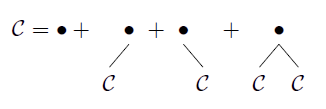
\includegraphics[width=.5\textwidth]{catalan_image.png}
        \end{center}
        \[C(z) = z + 2 z C(z) + z C^2(z)\]
        \[(n + 2) C_{n + 1} = 2(2n + 1) C_n \]
    \end{myexample}
\end{frame}

\begin{frame}{Interpretacje kombinatoryczne}
    \begin{myexample}
        \[(n + 2) C_{n + 1} = 2 (2n + 1) C_{n}\]

        \begin{center}
            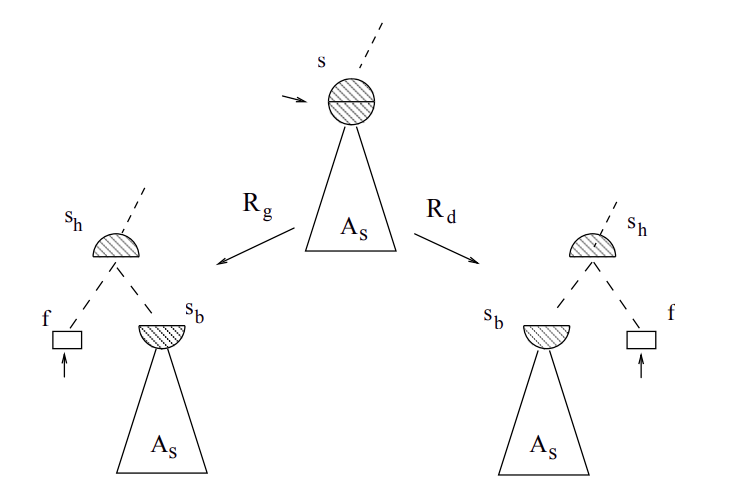
\includegraphics{catalan_interpretation.png}
        \end{center}
    \end{myexample}
\end{frame}

\section{Inspiracja}

\begin{frame}{Drzewa czarno-białe}
    \begin{columns}
        \column{.5\textwidth}
        \begin{mydefinition}
            Dozwolone krawędzie: 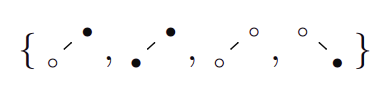
\includegraphics{bw.png}

            Korzeń czarny
        \end{mydefinition}

        \column{.5\textwidth}
        \begin{myexample}
            \begin{center}
                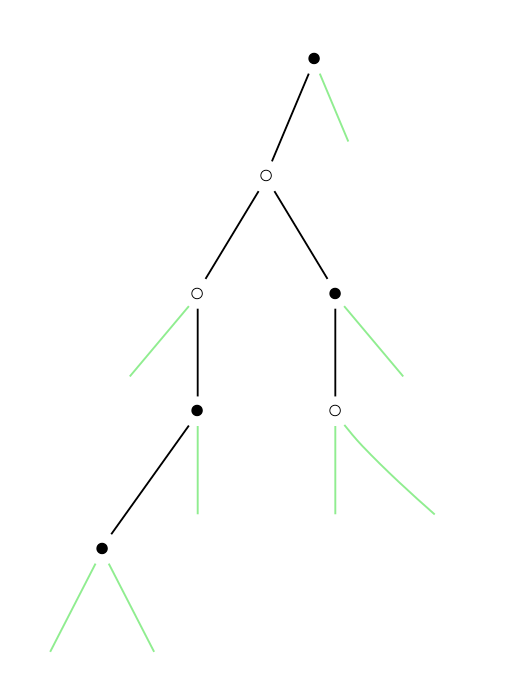
\includegraphics{bw_001.png}
            \end{center}
        \end{myexample}
    \end{columns}
\end{frame}

\begin{frame}{Drzewa bez zig-zagów}
    \begin{columns}
        \column{.5\textwidth}
        \begin{mydefinition}
            Zabroniony pattern:
            \begin{center}
                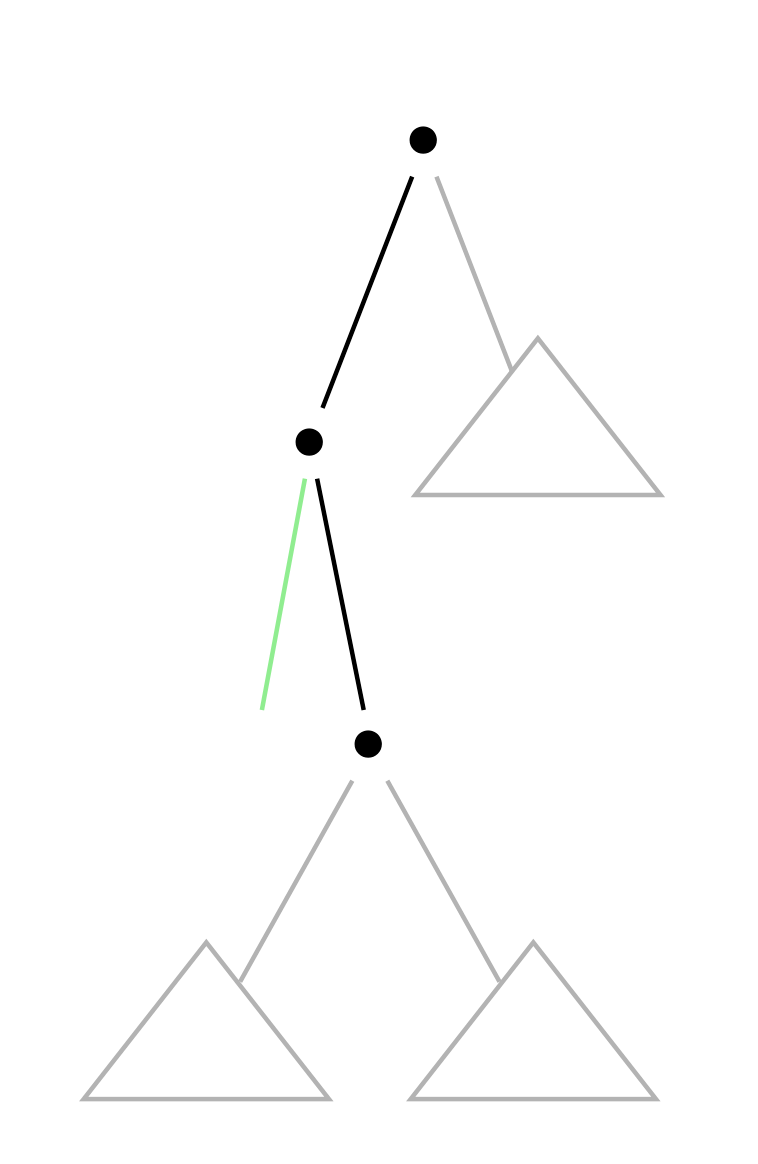
\includegraphics[height=\textwidth]{zigzag_forbid.png}
            \end{center}
        \end{mydefinition}

        \column{.5\textwidth}
        \begin{myexample}
            \begin{center}
                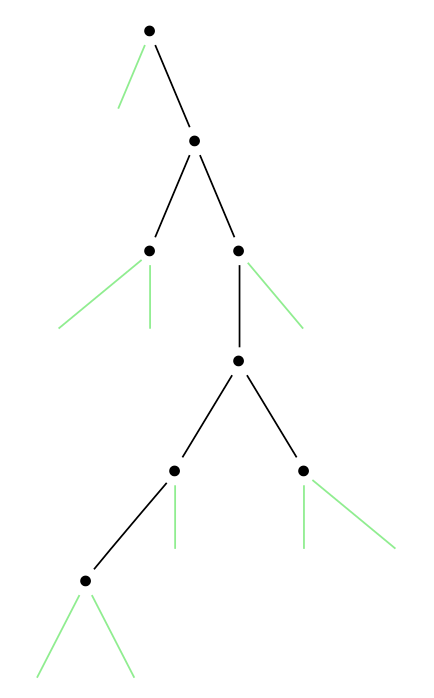
\includegraphics{zigzag_001.png}
            \end{center}
        \end{myexample}
    \end{columns}
\end{frame}

\begin{frame}{Drzewa termów lambda w notacji de Brujina}
    \begin{columns}
        \column{.5\textwidth}
        \begin{mydefinition}
            \begin{itemize}
                \item \(\forall n \in \mathbb{N}: n \text{ jest termem}\)
                \item \(P \text{ jest termem} \implies \lambda P \text{ jest termem}\)
                \item \(P, Q \text{ są termami} \implies P @ Q \text{ jest termem}\)
            \end{itemize}
        \end{mydefinition}

        \column{.5\textwidth}
        \begin{myexample}
            \begin{center}
                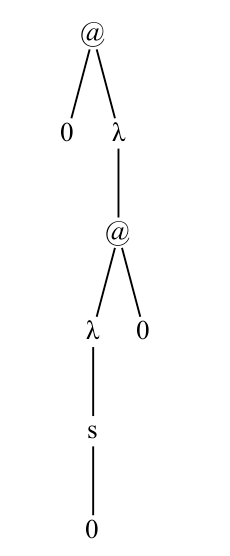
\includegraphics{lambda_001.png}
            \end{center}
        \end{myexample}
    \end{columns}
\end{frame}

\begin{frame}{Wspólna rekurencja holonomiczna}
    \begin{columns}
        \column{.6\textwidth}
        \begin{mydefinition}
            \[\begin{array}{rcl}
                (n + 1)L_n &=& (4n - 1)L_{n-1}\\
                           &-& (2n - 1)L_{n-2}\\
                           &-& L_{n-3}\\
                           &-& (n - 4)L_{n-4}
            \end{array}\]
        \end{mydefinition}

        \column{.4\textwidth}
        \begin{myexample}
            \begin{center}
                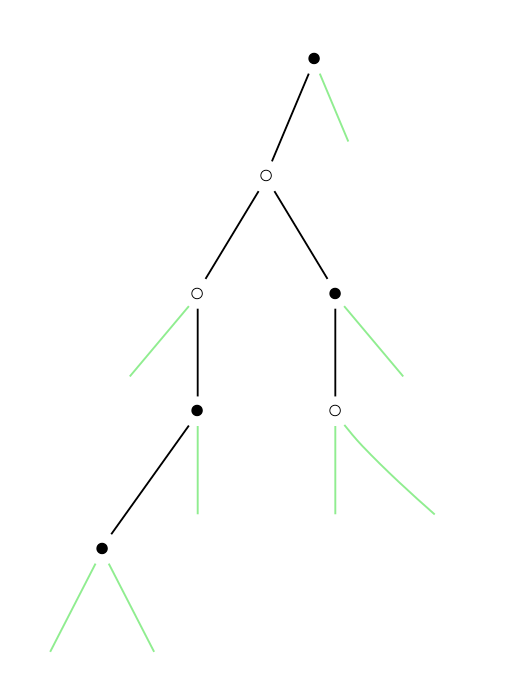
\includegraphics[width=.4\textwidth]{bw_001.png}%
                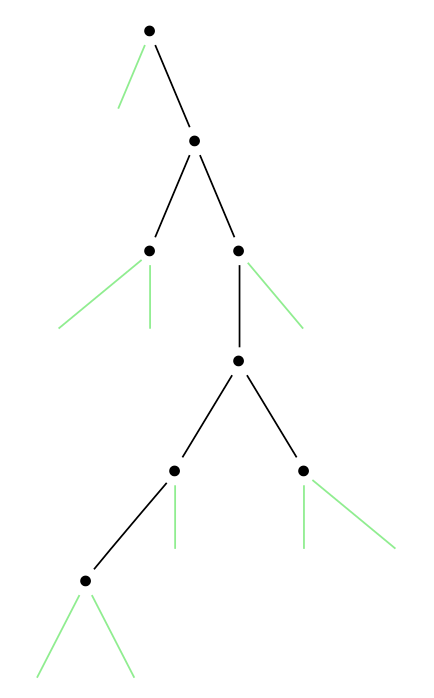
\includegraphics[width=.4\textwidth]{zigzag_001.png}%
                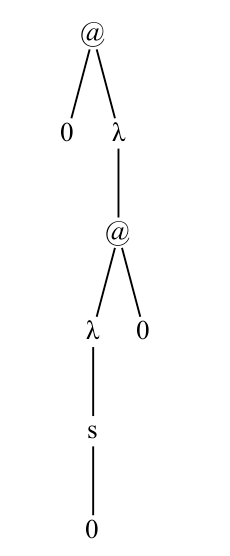
\includegraphics[width=.2\textwidth]{lambda_001.png}
            \end{center}
        \end{myexample}
    \end{columns}
\end{frame}

\begin{frame}{Wspólna rekurencja holonomiczna}
    \begin{mydefinition}
        \[\begin{array}{rcl}
                (n + |@|)\mathcal{L}_n &=& (2n - 3|\lambda| + 2|@|)\mathcal{L}_{n -|\lambda|}\\
                                       &-& (n - 3|\lambda| + |@|)\mathcal{L}_{n-2|\lambda|}\\
                                       &+& (4n - 6|0| - 2|@|)\mathcal{L}_{n-|0|-|@|}\\
                                       &-& (4n - 6|0| - 2|s| - 2|@|)\mathcal{L}_{n-|0|-|s|-|@|}\\
                                       &+& (2n - 2|s| + 2|@|)\mathcal{L}_{n-|s|}\\
                                       &-& (4n - 4|s| - 6|\lambda| + 4|@|)\mathcal{L}_{n-|s|-|\lambda|}\\
                                       &+& (2n - 2|s| - 6|\lambda| + 2|@|)\mathcal{L}_{n-|s|-2|\lambda|}\\
                                       &-& (n - 2|s| + |@|)\mathcal{L}_{n-2|s|}\\
                                       &+& (2n - 4|s| - 3|\lambda| + 2|@|)\mathcal{L}_{n-2|s|-|\lambda|}\\
                                       &-& (n - 2|s| - 3|\lambda| + |@|)\mathcal{L}_{n-2|s|-2|\lambda|}
        \end{array}\]
    \end{mydefinition}
\end{frame}

\section{Zastosowania}

\begin{frame}{Generowanie losowych drzew}
    \begin{myproductions}
        \[D_n = (n + 1)! C_n = \frac{(2n)!}{n!} = 2 (2n - 1) D_{n-1}\]
        \begin{center}
            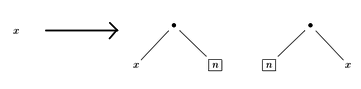
\includegraphics[width=.6\textwidth]{gen_001.png}
        \end{center}
    \end{myproductions}

    \begin{myexample}
        \begin{center}
            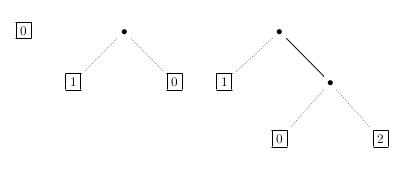
\includegraphics[width=.6\textwidth]{gen_002.png}
        \end{center}
    \end{myexample}
\end{frame}

\section{Cele pracy}

\begin{frame}{Cele pracy}
    \begin{itemize}
        \item Zebranie technik interpretacji kombinatorycznych rekurencji holonomicznych
        \item Próba interpretacji kombinatorycznej rekurencji holonomicznych dla drzew czarno-białych, drzew bez zig-zagów oraz drzew termów lambda
    \end{itemize}
\end{frame}

\end{document}
